\input format.tex

\usepackage{graphicx}
\graphicspath{{cores/}}

\usepackage{environ}
\usepackage{colortbl,array,booktabs}
\usepackage{tabularx}

\colorlet{TablaBordeSuperior}{topcolor}
\colorlet{TablaBordeInferior}{topcolor}
\colorlet{TablaCentroSuperior}{blue!1}
\colorlet{TablaCentroInferior}{blue!20}
\colorlet{FuenteCabeceraTabla}{white}

\newcolumntype{M}[1]{>{\centering\arraybackslash}m{#1}}
%\newcommand{\tabularxcolumn}[1]{>\arraybackslash}m{#1}}

\tcbset{rtab/.style={
freelance,
frame code={
 \path[top color=topcolor,bottom color=topcolor]
   ([yshift=-#1*(\baselineskip+2pt)]interior.north west) --
   ([yshift=-#1*(\baselineskip+2pt)]interior.north east) {[sharp corners]--
    ([yshift=3pt]interior.north east) --
    ([yshift=3pt]interior.north west)} -- cycle;

  },
interior code={},
 }
}

\newcommand\fuentecabecera[1]{\textcolor{black}{\textbf{#1}}}

\begin{document}

\vspace*{3mm}
%% 各章节
\setlength{\arrayrulewidth}{.2pt}
\fontsize{8.8pt}{11pt}\selectfont
\color{gray2}

\begin{center}
{\noindent\bf\sanhao 三、体重管理方案}
\end{center}

\vspace*{3mm}

\begin{spacing}{1.5}

\indent {\fontsize{8pt}{11pt}\selectfont 根据您目前检测结果,我们专属为您定制了精准减重方案,建议您严格按照方案执行,并在执行方案3个月后
定期复查,助您有效管理体重,保持苗条。}

\vspace*{2mm}

\noindent{\bf{微生态减重方案}}

\indent {\fontsize{8pt}{11pt}\selectfont 根据您本次肠道菌群检测结果,结合您的体质指数(BMI)、微生态平衡能力、瘦菌、胖菌等指标,为您制定如下个性化微生态减重方案: \\}
\indent {\fontsize{8pt}{11pt}\selectfont 建议您-。持续服用,能帮助减少肠道对糖类和脂肪的消化吸收,有利于控制体重及减重。\\}

\end{spacing}

\vspace*{3mm}

\noindent
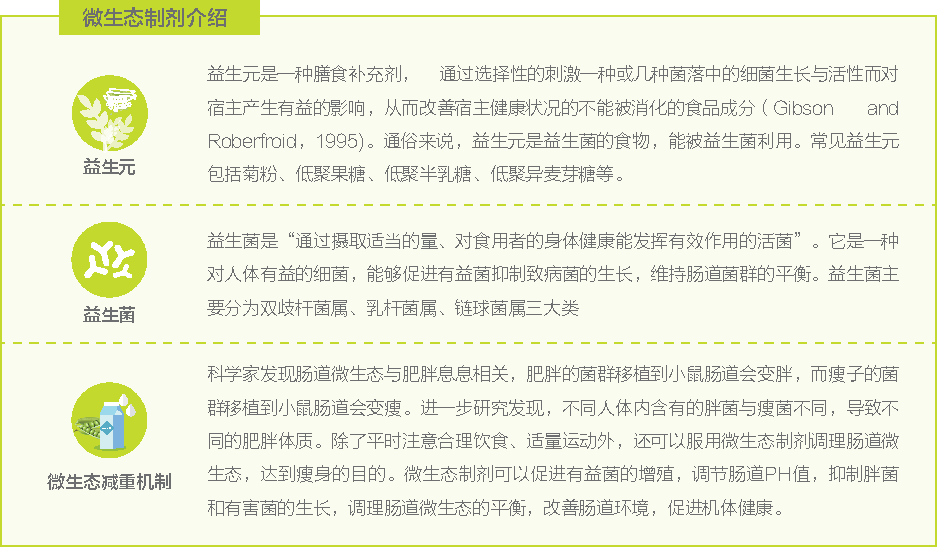
\includegraphics[width=\linewidth]{preprobiotics-intro.pdf}

\end{document}

